% Validating and Extending a Chapter-Aligned Moodle Engagement Metric
% Compile: pdflatex report.tex (twice)
\documentclass[11pt,a4paper]{article}

\usepackage[T1]{fontenc}
\usepackage[utf8]{inputenc}
\usepackage{lmodern}
\usepackage[margin=2.4cm]{geometry}
\usepackage{amsmath,amssymb}
\usepackage{graphicx}
\usepackage{booktabs}
\usepackage{array}
\usepackage{float}
\usepackage{caption}
\usepackage{subcaption}
\usepackage[round]{natbib}
\usepackage[hidelinks]{hyperref}

\graphicspath{{../outputs/figures/}}

\renewcommand{\figurename}{Fig.}
\captionsetup{font=small,labelfont=bf}
\captionsetup[sub]{font=small}
\setlength{\parskip}{0.35em}
\setlength{\parindent}{1.2em}
\bibliographystyle{plainnat}

\newcommand{\srcnote}{\par\smallskip{\footnotesize\textit{Source: author's analysis of UCL Moodle log data.}}}

\title{\bfseries Validating and Extending a Chapter-Aligned Moodle\\[2pt]
Engagement Metric Across STAT0002 and STAT0004\\[8pt]
\large Evidence from online, hybrid and in-person Moodle delivery cohorts}

\author{Research Internship Report\\
Department of Statistical Science, University College London}
\date{\today}

\begin{document}
\maketitle

\begin{abstract}
\noindent
Virtual learning environments such as Moodle record when students access course
resources, how often they return, and which types of activities they use. These
logs offer a scalable route to early student support, but simple click counts are
hard to interpret and supervised predictive models typically require historical
grade data. This report evaluates a theoretically grounded, chapter-aligned
engagement metric that summarises three behaviours for each student:
\textbf{Frequency} (the number of chapter-specific study sessions completed),
\textbf{Immediacy} (how promptly a student first accesses newly released chapter
material), and \textbf{Diversity} (the breadth of distinct resource types used
within a chapter). Each component is min-max scaled relative to peers within the
same chapter and teaching week, producing scores between 0 and~1, and the three
are added to form a chapter-level score, IDF $= F + I + D \in [0, 3]$. Summing
chapter scores across all material released by week~$t$ gives a cumulative
engagement measure that can be updated in real time without outcome data.
Building on the metric proposed by \citet{johnston2025}, this report applies
the fixed measure to five cohorts from two UCL undergraduate statistics modules:
STAT0002 (a first-year probability and statistics course) and STAT0004 (a
second-year programming and practical statistics course), together comprising $N = 1{,}291$
students and spanning online, hybrid and in-person delivery periods not used in
the original validation. The report asks whether the metric travels to new
cohorts, which component carries the most distinct information about final
grades, and whether the engagement--grade association is uniform across the grade
distribution or concentrated among lower-performing students.
Across the pooled cohorts, cumulative IDF shows a moderate positive association
with final grade ($r = 0.32$). Once the shared variance among the three
components is removed using a relative-importance decomposition, Diversity and
Immediacy account for more unique explained variance than Frequency at week~11
(mean shares of 37\%, 36\% and 27\%), even though all three correlate similarly
with grade in bivariate analysis. The engagement--grade association is also
stronger among lower-performing students: in every cohort, the slope at the
10th percentile of the grade distribution exceeds the median slope by an average
of 2.3 grade points per standard deviation of engagement, and indicator-specific
quantile models suggest that Immediacy is particularly important in the lower
tail. Together, the findings support using the metric for low-cost, supportive
monitoring rather than high-stakes prediction. Comparisons across delivery
periods remain descriptive because delivery mode is confounded with cohort and
academic year.
\end{abstract}

\section{Introduction}
Student engagement, the time and effort students devote to learning
activities, is widely linked to academic performance, satisfaction and
retention. In online and blended higher education, part of the \emph{behavioural}
dimension of engagement is recorded automatically by virtual learning
environments (VLEs): which resources students access, how often they return, and
how promptly they engage with newly released material. Moodle logs therefore
offer a scalable record of observed study behaviour, but they remain only a
proxy. They cannot observe offline study, motivation, attendance or the quality
of students' understanding \citep{henrie2015}.

This creates a practical measurement problem. Simple indicators such as total
clicks are easy to compute but difficult to interpret pedagogically; a high count
need not represent broad or sustained engagement \citep{fincham2019}. Threshold
systems can flag low activity, but their cut-offs are often arbitrary and may not
generalise. Supervised predictive models can be more flexible, yet they require
historical outcome data and can fail when moved to new modules, cohorts or
delivery contexts \citep{gasevic2016}. For early student support, an attractive
alternative is an interpretable metric that is grounded in engagement theory, can
be updated during the term, and can be validated without assuming that a low log
count is equivalent to low effort.

\citet{johnston2025} propose such a metric by adapting the earlier course-wide
engagement score of \citet{chong2019}. The original course-wide score combines
five indicators after the course has finished. Johnston et al. instead align the
measurement with how teaching material is released: for each student, chapter and
week, they compute Frequency, Immediacy and Diversity, scale each component
relative to peers, and add them into a chapter-level IDF score. Frequency captures
the volume of chapter-specific study sessions, Immediacy captures how soon a
student first engages with a chapter after it becomes available, and Diversity
captures the breadth of resource types accessed. Summing chapter scores over the
term gives a cumulative engagement trajectory that can be monitored in real time.

The present report is a secondary validation and extension of that fixed metric,
not a new metric-development exercise. It applies the chapter-aligned IDF measure
to five cohorts from two UCL undergraduate statistics modules. STAT0002 is a
first-year course introducing probability and statistical theory, represented
here by an online delivery (2020--21) and an in-person delivery (2022--23).
STAT0004 is a second-year programming and practical statistics course covering
statistical computing and data analysis, and is the only module spanning all three delivery
conditions: online (2020--21), hybrid (2021--22) and in-person (2022--23). These
five cohorts were not used in the original validation, providing a genuinely
independent test of the metric.

The analysis pursues two substantive questions. The first concerns component
importance: once the strong correlations among Frequency, Immediacy and Diversity
are accounted for, which component carries the most unique information about
final grades? A relative-importance decomposition due to \citet{lindeman1980},
known as the LMG method, addresses this by averaging each predictor's
contribution to explained variance over all possible orderings in which the
three components could enter a regression model. The second question asks whether
the engagement--grade association is uniform across the grade distribution or
stronger among students already at academic risk. Quantile regression estimates
the slope between engagement and grade separately at different percentiles of the
grade distribution, making it possible to ask whether low engagement is more
consequential for lower-performing students than for the average student.
Supporting analyses assess the overall pooled association, signal timing,
engagement trajectories, early-warning precision, assessment-component alignment
and robustness to analytic choices. Delivery-period comparisons are treated as
descriptive boundary checks rather than causal tests because delivery mode is
perfectly confounded with cohort and academic year.

\section{Background and metric context}
Online behavioural engagement refers to observable, sustained interaction with
learning activities in a digital environment. Engagement theory distinguishes
behavioural, emotional and cognitive forms of involvement; Moodle logs capture
primarily the behavioural dimension, participation, effort and attention to
academic tasks, rather than motivation or understanding
\citep{fredricks2004,henrie2015,martinborup2022}. It is only a \emph{proxy} for learning: logs
record what happens inside the VLE, not offline study, in-person attendance or
the quality of students' reasoning. Even so, when behavioural engagement is
measured coherently and validated against academic outcomes, it can support
timely monitoring and targeted support.

The course-wide metric of \citet{chong2019} combines five indicators (Immediacy,
Frequency, Diversity, Recency and Interval) into a single retrospective score
aggregated across an entire course. That design is useful for end-of-term analysis
but poorly suited to weekly monitoring, and it treats the course as homogeneous
rather than aligned with its chapter structure. For real-time monitoring this is
problematic: a student may be on schedule with newly released material while
having little activity on later chapters that are not yet relevant, or may return
frequently to old material without keeping pace with current content.

\citet{johnston2025} address this by moving from a course-wide score to a
chapter-aligned score. At each week $t$, and for each released chapter $k$, three
raw indicators are calculated from chapter-specific study sessions:
\textbf{Frequency}, the number of study sessions associated with the chapter;
\textbf{Immediacy}, the delay between the chapter's first observed availability
and the student's first chapter-specific session, transformed so earlier access
receives a higher score; and \textbf{Diversity}, the number of distinct Moodle
activity or resource types accessed within that chapter. Each raw indicator is min-max scaled across all students for the same chapter
$k$ and week $t$, placing it on a common $[0,1]$ scale relative to peers. For
example, the scaled Immediacy indicator is
\[
  I_{k,t}^{(i)} =
  \frac{\tilde{I}_{k,t}^{(i)} - \min_{i}\,\tilde{I}_{k,t}^{(i)}}
       {\max_{i}\,\tilde{I}_{k,t}^{(i)} - \min_{i}\,\tilde{I}_{k,t}^{(i)}},
\]
and the same transformation is applied to $\tilde{F}$ and $\tilde{D}$. A student
who scores 1 on all three components engaged with the chapter earlier, more
frequently, and across a broader range of resource types than any of their peers.
The chapter-level IDF score is then the simple sum
\[
IDF_{k,t}^{(i)} = F_{k,t}^{(i)} + I_{k,t}^{(i)} + D_{k,t}^{(i)} \in [0,3],
\]
so a high score means that a student engages often, early and broadly with that
chapter. Chapter scores are then summed over released chapters to obtain an
overall cumulative engagement measure for student $i$ at week $t$. Recency and
Interval are excluded from the real-time version because they become unstable
when measured before the course has finished.

Chapter alignment matters because engagement is most interpretable when measured
in step with how material is released. For early-warning use, practitioners also
need to understand the recall--precision trade-off: flagging the lowest-engagement
students may capture many who ultimately struggle, but also many who would have
succeeded without intervention \citep{conijn2017}. The present report takes the
metric definition as given and focuses on how it behaves on new UCL cohorts and
what additional diagnostic insight can be extracted from its components and
related temporal patterns.

\section{Data and engagement measures}
The analysis uses five module-year deliveries from two undergraduate statistics
modules at University College London. STAT0002 is a first-year foundations module
represented here by an online cohort (2020--21) and an in-person cohort
(2022--23). STAT0004 is a second-year module and the only module in this dataset
spanning all three delivery conditions: online (2020--21), hybrid (2021--22) and
in-person (2022--23). Each delivery covers eleven teaching weeks with up to ten
labelled chapters. Final grades are recorded on a 0--100 scale; grades below 50
were treated as low performance, and grades below 40 as failure. Students with
a recorded grade of zero, typically reflecting exam absence, were excluded.

Table~\ref{tab:inventory} summarises the cohorts. The main engagement--grade
sample comprises $N=1{,}291$ students with both engagement records and valid
final grades after exclusions. The latent trajectory analysis below uses
$N=1{,}290$ students with complete weekly engagement profiles suitable for class
assignment; the difference of one student reflects missing weekly coverage in
the trajectory model, not an error in the cohort inventory.

\begin{table}[H]
\centering
\caption{Cohort inventory for the main engagement--grade sample ($N=1{,}291$).}
\label{tab:inventory}
\small
\begin{tabular}{lllrrrr}
\toprule
Module & Year & Condition & $N$ & Mean (SD) & \%\,$<50$ & \%\,$<40$ \\
\midrule
STAT0002 & 2020--21 & Online    & 342 & 66.8 (13.8) & 9.9  & 1.8 \\
STAT0002 & 2022--23 & In-person & 268 & 67.4 (13.0) & 10.4 & 2.6 \\
STAT0004 & 2020--21 & Online    & 312 & 62.7 (12.2) & 12.5 & 2.9 \\
STAT0004 & 2021--22 & Hybrid    & 172 & 71.9 (8.8)  & 1.7  & 0.0 \\
STAT0004 & 2022--23 & In-person & 197 & 70.6 (11.3) & 3.6  & 1.0 \\
\midrule
\multicolumn{3}{l}{\textbf{Total}} & \textbf{1{,}291} & & & \\
\bottomrule
\end{tabular}
\srcnote
\end{table}

Two design features constrain interpretation. First, the share of low-performing
students varies widely across cohorts (from 1.7\% to 12.5\%), which limits how
sharply any early-warning flag can perform in the highest-achieving deliveries.
Second, delivery condition is \textbf{perfectly confounded} with academic year and
cohort: online corresponds to 2020--21, hybrid to 2021--22, and in-person to
2022--23. Comparisons across conditions therefore describe different module-year
contexts rather than randomly assigned delivery modes, and no causal claim about
online, hybrid or in-person delivery can be supported.

The modules also differed in assessment structure. STAT0002 in-person records
separate exam, participation and peer-marking components; STAT0004 deliveries
include coursework and quiz marks, with a group component in the in-person year.
This matters because Moodle engagement may align more closely with
individual or exam-style assessment than with group, peer-marked or participation
components. Where component marks were available, this report therefore analyses
whether the engagement metric correlates more strongly with individually assessed
work than with collaborative or peer-assessed components.

The two modules also differ in the strength of the engagement--grade link across
deliveries. STAT0002 cohorts show end-of-term correlations of $r=0.28$--$0.41$,
whereas STAT0004 ranges from $r=0.19$ to $r=0.30$. As interpretive context, the
two modules may differ in ways that affect how well Moodle activity proxies study
behaviour; several factors may contribute, though they cannot be disentangled in
this observational design. STAT0002 is a first-year foundations module with
substantial individually assessed exam weight, where sustained access to lecture
materials and problem sheets may track preparation more directly. STAT0004 is a
second-year module with greater student autonomy, more coursework and
group-assessment weighting, and possibly more study away from Moodle. Each of
these factors would weaken the observable link between VLE logs and final outcomes. How
tightly Moodle resources are organised by chapter may also matter: where chapter
labelling aligns less clearly with assessed work, a chapter-aligned metric would
legitimately carry less outcome signal, as \citet{johnston2025} report for less
structured courses.

\subsection{Engagement feature construction}
The supplied engagement table contains weekly chapter-level contribution columns
for Frequency, Immediacy and Diversity. These are the operational form of the
Johnston et al. IDF components used in this report: each column corresponds to a
student--week--chapter contribution for one component. Before modelling, the
data were checked to clarify their time semantics. A reconstruction from the raw
Moodle event log showed that the supplied contribution values behave as
\emph{per-week increments}, not as already cumulative totals. This matters
because the paper's real-time metric is cumulative up to week $t$; therefore the
analysis must first build weekly totals and then accumulate them explicitly.

For each student and week, contribution values were summed across released
chapters to obtain weekly Frequency, Immediacy and Diversity totals. The weekly
composite was then defined additively as
\[
\mathrm{IDF}_\mathrm{week} = \mathrm{freq}_\mathrm{week} +
\mathrm{imm}_\mathrm{week} + \mathrm{div}_\mathrm{week},
\]
and cumulative measures were obtained by summing across weeks:
separately for Frequency, Immediacy, Diversity and the composite IDF:
\[
  \mathrm{cum\_IDF}_{i,t} = \sum_{s=1}^{t}\mathrm{IDF}_{\mathrm{week},i,s}.
\]
This
additive definition follows the chapter-level formulation of
\citet{johnston2025}; it is not a multiplicative composite and no outcome data
are used to create the engagement measures. The reconstruction check confirmed
that the supplied contributions are most consistent with the intended per-week
Frequency and Diversity definitions, while Immediacy is retained as supplied
because it depends on first-access timing and release-date assumptions.

For extension analyses, additional timing and regularity features were derived
from event logs (for example, variation in weekly activity and gaps between
sessions). Latent-class mixed models were also fitted to normalised weekly
cumulative IDF curves to identify distinct engagement trajectories over the term.

\section{Methods}

\subsection{Overall association with final grade}
Within each cohort, Spearman rank correlations were computed between cumulative
engagement and final grade at each week and at the end of term. To synthesise
evidence across cohorts, cohort-specific correlations were pooled using a
random-effects meta-analysis implemented with \texttt{metafor}
\citep{viechtbauer2010}, reporting the pooled correlation, confidence interval
and $I^2$ heterogeneity statistic. Complementing rank-based evidence, a
mixed-effects model was fitted with final grade as the outcome and standardised
cumulative IDF as the predictor, allowing the slope to vary by cohort. This
expresses the association on the grade scale in points per one standard deviation
of engagement.

\subsection{Component importance: relative-importance decomposition}
Because Frequency, Immediacy and Diversity are strongly correlated (mean pairwise
$|r| \approx 0.75$--$0.83$; variance inflation factors VIF $\approx 2.6$--$4.4$
at weeks~6 and~11), ordinary partial regression coefficients are unstable under
collinearity and can even reverse sign across cohorts. To obtain stable estimates
of each component's unique contribution, the Lindeman--Merenda--Gold (LMG) method
\citep{lindeman1980} is used. LMG partitions the model $R^2$ from the regression
of final grade on Frequency, Immediacy and Diversity into additive shares, one
per predictor, by averaging each predictor's marginal contribution to $R^2$ over
all possible orderings in which the three components enter the model. Because
averaging over orderings removes the dependence on any single variable ordering,
the resulting shares are stable under collinearity and sum exactly to the total
model $R^2$. Shares are computed separately for each cohort at weeks~6 and~11 and
then averaged. Bivariate Spearman rank correlations from meta-analysis provide a
complementary contrast: they show how each component associates with grade in
isolation, before removing shared variance.

\subsection{Heterogeneity across the grade distribution: quantile regression}
To test whether engagement matters equally for all students or more strongly for
lower-performing students, quantile regression \citep{koenker1978} is used. The
model takes the form
\[
  \mathrm{grade}_i = \beta_0(\tau) + \beta_1(\tau)\,z_{\mathrm{IDF},i} +
  \varepsilon_i(\tau),
\]
where $z_{\mathrm{IDF},i}$ is cumulative engagement standardised within cohort
and week, $\tau$ ranges over $\{0.1, 0.25, 0.5, 0.75, 0.9\}$, and
$\beta_1(\tau)$ gives the grade-point change per one standard deviation of
engagement at that quantile of the grade distribution. If engagement matters
equally for all students, $\beta_1(\tau)$ should be roughly constant across
$\tau$; if it matters more for lower-performing students, the slope at $\tau=0.1$
should exceed that at $\tau=0.5$ (the median). The descriptive contrast
$\beta_1(0.1) - \beta_1(0.5)$ is supplemented by bootstrap confidence intervals
based on 500 student-level resamples per cohort. Indicator-specific quantile
models (one of Frequency, Immediacy or Diversity at a time) identify which
component drives lower-tail associations. Analyses are conducted at weeks~6
and~11.

\subsection{Timing and early-course usefulness}
Weekly Spearman correlations between cumulative engagement and final grade were
tracked across the term to assess how early the association emerges. For each
cohort, a bootstrap procedure identified the earliest week at which the
correlation was statistically indistinguishable from its end-of-term value,
providing a practical sense of when the signal stabilises.

\subsection{Early-warning performance}
Students were grouped into engagement quintiles at selected weeks, and the
distribution of final grades within each quintile was examined. The bottom
engagement quintile was treated as a risk flag and evaluated using the area under
the ROC curve (AUC), recall and precision for identifying students scoring below
50\% at the end of term. These complementary measures are reported because AUC
alone can look favourable in imbalanced samples while obscuring the proportion of
flagged students who ultimately require support \citep{conijn2017,johnston2025}.

\subsection{Assessment-component validity}
Where separate assessment marks were available, engagement was correlated with
each component and Steiger's test for dependent correlations was used to compare
whether engagement aligns more strongly with individually assessed work (exams,
quizzes) than with group- or peer-marked components \citep{steiger1980,almond2009}.

\subsection{Temporal regularity and trajectory analysis}
Timing and regularity features were added to models already containing F, I and
D to test whether \emph{how} students engage over time adds information beyond
\emph{how much} and \emph{how broadly} they engage. Separately, latent-class mixed
models were applied to weekly cumulative IDF profiles to identify groups of
students following distinct engagement trajectories and to compare their final
grades. To assess operational usefulness, end-of-term class labels were compared
with early assignments made by matching each student's partial weekly profile
(weeks 1--$w$) to the corresponding segment of the end-of-term class centroids.
Latent-class mixed models were estimated using the \texttt{lcmm} framework
\citep{proustlima2017}.

\subsection{Robustness checks}
The main conclusions were examined under degree-programme adjustment,
false-discovery-rate correction using the Benjamini--Hochberg procedure across
weekly association tests, alternative bounded outcome specifications, and
variation in the at-risk engagement threshold. These
checks were kept brief and interpreted in the context of the primary findings
rather than treated as a separate technical audit.

\section{Results}
Results are reported first for the overall association between cumulative
engagement and final grade, then for the component and grade-distribution
analyses, before turning to timing, trajectories, assessment alignment,
early-warning performance and robustness.

\subsection{Overall engagement--grade association}
Across all five cohorts, cumulative engagement is positively and moderately
associated with final grade. The random-effects pooled rank correlation for
cumulative IDF at week 11 is $r=0.32$ (95\% CI $[0.25, 0.38]$), with
low-to-moderate heterogeneity across cohorts ($I^2=39\%$). Frequency, Immediacy
and Diversity show similar pooled associations when analysed separately
(Table~\ref{tab:meta}). On the grade scale, the mixed-effects estimate
corresponds to approximately 3.8 grade points per one standard deviation increase
in engagement. Figure~\ref{fig:forest} shows that every cohort lies above zero,
but the association is far from perfect prediction: engagement is a useful but
imperfect proxy for academic performance.

\begin{table}[H]
\centering
\caption{Pooled rank correlations and mixed-effects slopes at week 11.}
\label{tab:meta}
\small
\begin{tabular}{lcccc}
\toprule
Indicator & Pooled $r$ [95\% CI] & $I^2$ & Slope (SE) & Moderator $p$ \\
\midrule
Frequency & 0.28 [0.22, 0.34] & 27\% & 3.36 (0.53) & 0.92 \\
Immediacy & 0.30 [0.24, 0.37] & 37\% & 3.63 (0.58) & 0.88 \\
Diversity & 0.31 [0.24, 0.37] & 33\% & 3.62 (0.53) & 0.87 \\
\textbf{IDF} & \textbf{0.32 [0.25, 0.38]} & \textbf{39\%} & \textbf{3.79 (0.58)} & 0.89 \\
\bottomrule
\end{tabular}
\srcnote
\end{table}

\begin{figure}[H]
\centering
\includegraphics[width=0.82\textwidth]{12_forest_IDF.png}
\caption{Cohort-specific and pooled week-11 correlations between cumulative IDF
engagement and final grade. All cohorts show positive associations; the
random-effects estimate summarises the overall moderate engagement--grade
relationship.}
\label{fig:forest}
\end{figure}

STAT0002 deliveries show stronger cohort-level associations than STAT0004
($r=0.28$--$0.41$ versus $r=0.19$--$0.30$), consistent with the module-level
patterns noted in Section~3. The pooled estimate nonetheless remains positive and
moderate because every cohort contributes in the same direction.

When students are ranked by cumulative engagement and grouped into quintiles,
final grades tend to rise across successive quintiles, particularly in STAT0002,
where quintile separation is clearest (Figure~\ref{fig:quintile}). At weeks 3 and 6,
the lowest-engagement quintile is the group whose grade distribution most often
approaches or crosses the 50\% low-performance threshold, while the
highest-engagement quintile consistently shows the strongest outcomes. Separation
between adjacent middle quintiles is weaker, which is consistent with a monotone
but noisy relationship rather than sharp boundaries between moderate engagement
levels. Together, the pooled correlation, positive cohort-level associations and
quintile patterns support the conclusion that the metric \emph{travels} to these
new module-year contexts with a moderate, robust association.

\begin{figure}[H]
\centering
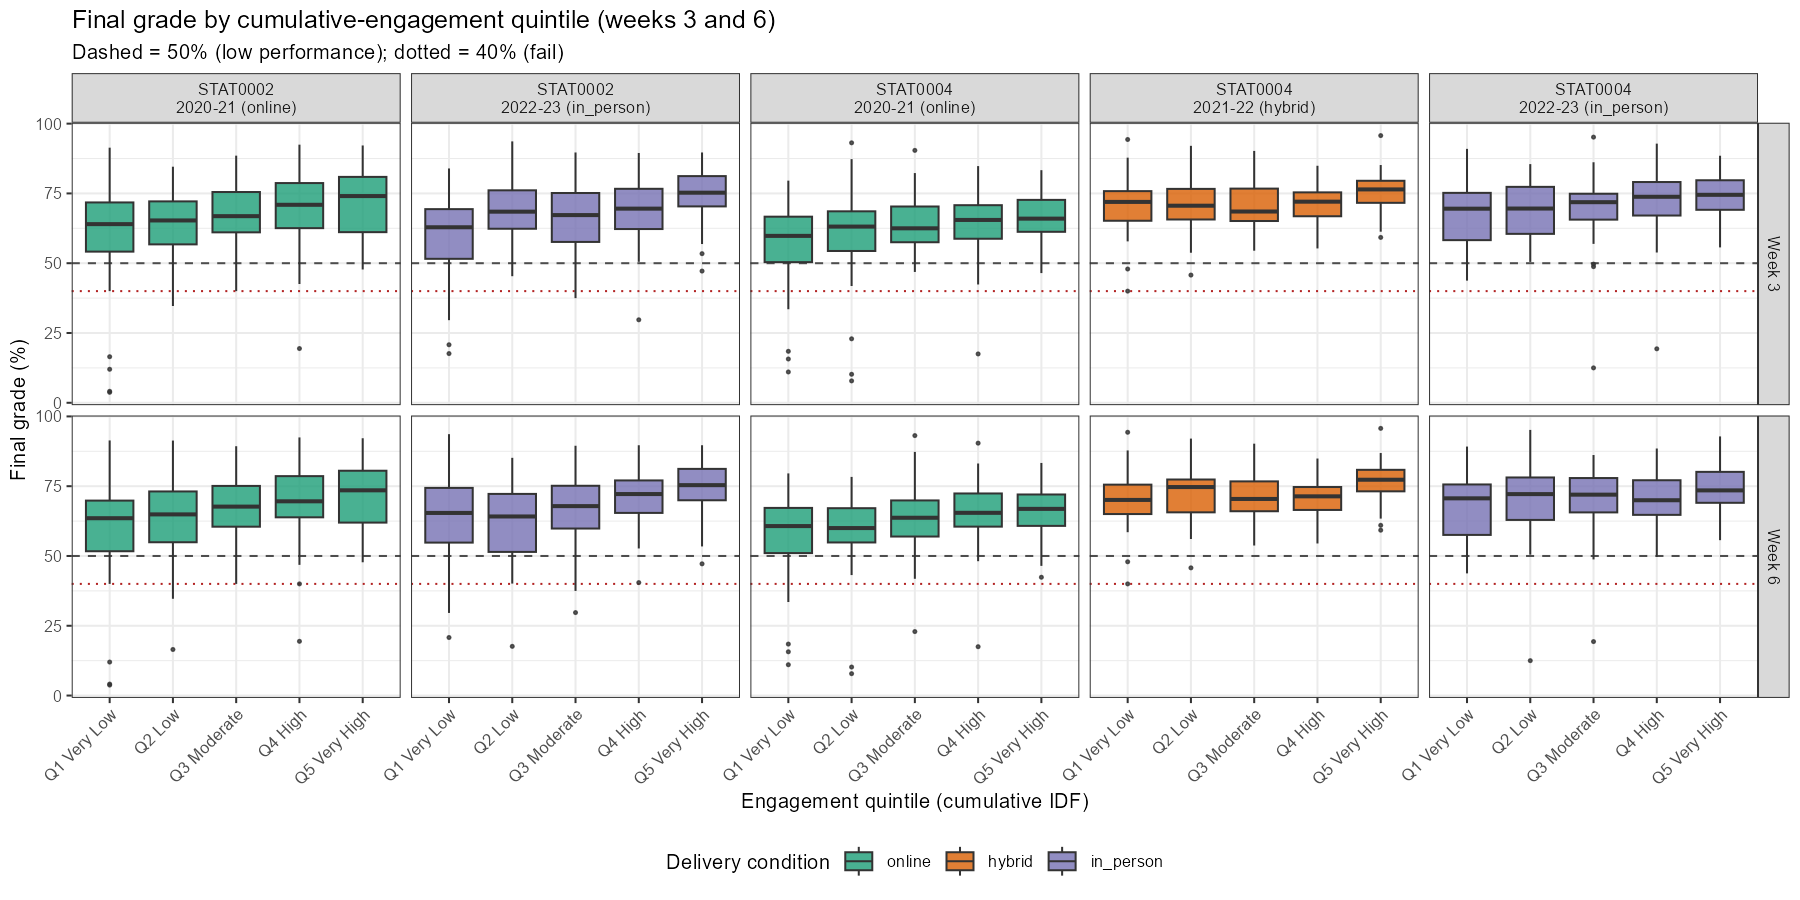
\includegraphics[width=0.95\textwidth]{06_quintile_boxplots_w3_w6.png}
\caption{Final-grade distributions by engagement quintile at weeks 3 and 6.}
\label{fig:quintile}
\end{figure}

\subsection{Component importance}
Treating engagement as a single composite score confirms that it relates to
grades, but obscures \emph{which} learning behaviours carry unique predictive
information. Frequency (how often students interact), Diversity (the variety of
resource types accessed) and Immediacy (how promptly students engage with newly
released content) are strongly correlated within cohorts: mean pairwise
$|r| \approx 0.75$--$0.83$, with variance inflation factors between 2.6 and 4.4
at weeks~6 and~11. Under such collinearity, ordinary multiple-regression
coefficients are unstable and can even change sign across cohorts; a method that
partitions explained variance fairly is required.

\paragraph{Bivariate contrast.}
Bivariate pooled rank correlations at week~11 show similar associations
for all three indicators when analysed separately: $r=0.28$ (Frequency),
$r=0.30$ (Immediacy) and $r=0.31$ (Diversity; Table~\ref{tab:meta}). Taken alone,
this would suggest that all components matter equally. The LMG results show that
this is misleading once shared variance is removed.

\paragraph{End-of-term results.}
At end-of-term (week~11), Diversity accounts for the largest mean share of
explained variance (37\%), Immediacy is intermediate (36\%), and Frequency the
smallest (27\%). Frequency has the smallest LMG share in every cohort
(Table~\ref{tab:importance}, Figure~\ref{fig:lmg}). Cohort-level patterns vary:
Immediacy dominates in STAT0002 online (45\%), whereas Diversity dominates in
STAT0004 online and in-person (45\% and 42\% respectively).

\begin{table}[H]
\centering
\caption{LMG relative-importance shares (\%) at week 11.}
\label{tab:importance}
\small
\begin{tabular}{lccc}
\toprule
Cohort & Frequency & Immediacy & Diversity \\
\midrule
STAT0002 online    & 28 & 45 & 27 \\
STAT0002 in-person & 28 & 36 & 36 \\
STAT0004 online    & 23 & 32 & 45 \\
STAT0004 hybrid    & 31 & 32 & 38 \\
STAT0004 in-person & 25 & 33 & 42 \\
\midrule
\textbf{Mean} & \textbf{27} & \textbf{36} & \textbf{37} \\
\bottomrule
\end{tabular}
\srcnote
\end{table}

\begin{figure}[H]
\centering
\includegraphics[width=0.95\textwidth]{13_lmg_importance.png}
\caption{LMG relative-importance shares for Frequency, Immediacy and Diversity by
cohort at weeks~6 (left) and~11 (right). Diversity and Immediacy typically account
for more unique explained variance than Frequency.}
\label{fig:lmg}
\end{figure}

\paragraph{Mid-term results.}
The same decomposition at week~6, the course midpoint and a common decision point
for early support, shows a broadly similar ranking: Diversity remains the top
contributor on average (39\%), with Immediacy lowest (24\%) and Frequency
intermediate (37\%). One cohort (STAT0004 in-person) assigns a larger week~6
share to Frequency (50\%), but Frequency never ranks first at week~11 in any
cohort. The pooled pattern supports interpreting breadth of resource use as the
most consistent unique signal, with promptness also carrying substantial
information, especially in first-year STAT0002.

\begin{table}[H]
\centering
\caption{LMG relative-importance shares (\%) at week 6.}
\label{tab:importance_wk6}
\small
\begin{tabular}{lccc}
\toprule
Cohort & Frequency & Immediacy & Diversity \\
\midrule
STAT0002 online    & 31 & 37 & 32 \\
STAT0002 in-person & 35 & 22 & 43 \\
STAT0004 online    & 32 & 25 & 43 \\
STAT0004 hybrid    & 38 & 18 & 43 \\
STAT0004 in-person & 50 & 17 & 33 \\
\midrule
\textbf{Mean} & \textbf{37} & \textbf{24} & \textbf{39} \\
\bottomrule
\end{tabular}
\srcnote
\end{table}

\begin{figure}[H]
\centering
\includegraphics[width=0.72\textwidth]{13_lmg_pooled_bootstrap.png}
\caption{Pooled mean LMG importance shares across cohorts at weeks~6 and~11.}
\label{fig:lmg_pooled}
\end{figure}

\subsection{Variation across the grade distribution}
A single average association, whether from OLS or Spearman correlation, can
hide whether engagement is more consequential for students already at academic
risk. Quantile regression addresses this by estimating separate slopes at
different points in the grade distribution.

\paragraph{Composite engagement.}
At week~11, the IDF slope is steeper at $\tau=0.1$ than at $\tau=0.5$ in
\textbf{every cohort} (Table~\ref{tab:quantile}). On average, the lower-tail
slope exceeds the median slope by 2.3 grade points per standard deviation of
engagement. Slopes generally decrease from $\tau=0.1$ through $\tau=0.5$ to
$\tau=0.9$, indicating that engagement variation is most consequential among
lower-performing students. For example, in STAT0002 in-person the slope is 7.9
points at $\tau=0.1$ versus 5.0 at the median and 3.0 at $\tau=0.9$. STAT0004
hybrid shows the smallest tail excess (0.6 points), suggesting cohort-specific
heterogeneity in how sharply the lower tail diverges.

Student-level bootstrap confidence intervals for $\beta_1(0.1) - \beta_1(0.5)$
confirm the pattern in two of five cohorts at week~11 (STAT0002 and STAT0004
in-person); in the remaining cohorts the point estimates are positive but
intervals are wide (Table~\ref{tab:quantile_boot}). At week~6, three cohorts show
positive descriptive contrasts and one (STAT0004 in-person) has a bootstrap
interval excluding zero.

\begin{table}[H]
\centering
\caption{Quantile-regression slopes for cumulative IDF at week 11 (grade points per +1 SD).}
\label{tab:quantile}
\small
\begin{tabular}{lcccc}
\toprule
Cohort & $\tau=0.1$ & $\tau=0.5$ & $\tau=0.9$ & $\tau_{0.1}-\tau_{0.5}$ \\
\midrule
STAT0002 online    & 5.32 & 3.22 & 2.58 & 2.11 \\
STAT0002 in-person & 7.88 & 5.04 & 2.96 & 2.84 \\
STAT0004 online    & 6.06 & 3.15 & 2.17 & 2.91 \\
STAT0004 hybrid    & 3.26 & 2.66 & 1.34 & 0.59 \\
STAT0004 in-person & 3.97 & 1.10 & 1.28 & 2.88 \\
\bottomrule
\end{tabular}
\srcnote
\end{table}

\begin{table}[H]
\centering
\caption{Bootstrap 95\% CI for $\tau_{0.1}-\tau_{0.5}$ contrast (week 11).}
\label{tab:quantile_boot}
\small
\begin{tabular}{lccc}
\toprule
Cohort & Contrast & 95\% CI & CI $> 0$? \\
\midrule
STAT0002 online    & 2.11 & [$-$1.60, 4.79] & No \\
STAT0002 in-person & 2.84 & [0.16, 5.54]   & Yes \\
STAT0004 online    & 2.91 & [$-$0.85, 4.77] & No \\
STAT0004 hybrid    & 0.59 & [$-$2.62, 4.49] & No \\
STAT0004 in-person & 2.88 & [0.26, 5.77]   & Yes \\
\bottomrule
\end{tabular}
\srcnote
\end{table}

\begin{figure}[H]
\centering
\includegraphics[width=0.95\textwidth]{11_quantile_idf.png}
\caption{Quantile-regression slopes of final grade on cumulative IDF at week~11,
with 95\% confidence intervals, by cohort.}
\label{fig:quantile}
\end{figure}

\begin{figure}[H]
\centering
\includegraphics[width=0.95\textwidth]{11_quantile_idf_wk6.png}
\caption{Quantile-regression slopes at week~6 (mid-term). The lower-tail pattern
is visible in most cohorts by the course midpoint.}
\label{fig:quantile_wk6}
\end{figure}

\paragraph{Indicator-specific associations.}
Univariate quantile regression (one indicator at a time) shows that \textbf{Immediacy}
has the largest mean slope at $\tau=0.1$ across cohorts at week~11 (4.9 grade
points per SD), followed by Diversity and Frequency
(Figure~\ref{fig:quantile_uni}). This complements the LMG finding that Diversity
carries the most unique variance in multivariate models: promptness appears
especially salient for distinguishing outcomes among lower-performing students
when indicators are considered separately.

\begin{figure}[H]
\centering
\includegraphics[width=0.85\textwidth]{11_quantile_univariate.png}
\caption{Mean univariate quantile-regression slopes by indicator (weeks~6 and~11;
mean across five cohorts). Larger coefficients at low $\tau$ indicate stronger
associations among lower-performing students.}
\label{fig:quantile_uni}
\end{figure}

\subsection{Timing and stabilisation}
Bootstrap stabilisation analysis asks whether additional weeks materially change
the engagement--grade correlation, not whether the correlation is already strong
(Table~\ref{tab:stab}, Figure~\ref{fig:stab}). In four cohorts, the weekly
correlation is statistically close to its end-of-term value from week 1 or 2,
but this sometimes reflects a relatively flat and modest signal rather than
impressive early predictive power. For example, STAT0004 in-person stabilises
early yet has a weak end-of-term association ($r=0.19$); STAT0004 hybrid
similarly stabilises at week 1 with $r=0.23$. By contrast, STAT0002 in-person
shows a strengthening association that does not stabilise until around week 9,
reaching the strongest cohort-level correlation ($r \approx 0.41$), suggesting
that later engagement adds meaningful information in that delivery. Stabilisation
timing and association strength should therefore be read separately: early
stabilisation does not guarantee a strong early-warning signal.

\begin{table}[H]
\centering
\caption{Stabilisation week and end-of-term IDF--grade correlation.}
\label{tab:stab}
\small
\begin{tabular}{lcc}
\toprule
Cohort & Stabilisation week & End-of-term $r$ \\
\midrule
STAT0002 online    & 2 & 0.28 \\
STAT0002 in-person & 9 & 0.41 \\
STAT0004 online    & 1 & 0.30 \\
STAT0004 hybrid    & 1 & 0.23 \\
STAT0004 in-person & 1 & 0.19 \\
\bottomrule
\end{tabular}
\srcnote
\end{table}

\begin{figure}[H]
\centering
\includegraphics[width=0.92\textwidth]{15_stabilisation.png}
\caption{Weekly Spearman correlation between cumulative engagement and final grade
by cohort, with bootstrap stabilisation week marked. Early stabilisation can
reflect a flat, modest signal as well as a strong one; compare stabilisation week
with end-of-term $r$ in Table~\ref{tab:stab}.}
\label{fig:stab}
\end{figure}

\subsection{Engagement trajectories}
Latent-class analysis identifies three weekly cumulative IDF trajectory types:
low-steady, high-steady and mid-variable (Figure~\ref{fig:traj}). Final grades
differ markedly across classes (Kruskal--Wallis $p = 2.6 \times 10^{-17}$). The
high-steady class averages 72.9, compared with 63.2 for the low-steady class: a
gap of about 9.7 grade points. The low-steady class also contains the highest
share of low performers (15.7\%). Sustained engagement \emph{patterns} over the
term therefore separate outcomes more sharply than a single cumulative score at
one time point, and identify a group whose profile is persistently low rather
than temporarily quiet.

\begin{table}[H]
\centering
\caption{Trajectory classes and grade outcomes ($N=1{,}290$).}
\label{tab:traj}
\small
\begin{tabular}{lccc}
\toprule
Class & $N$ & Mean grade & \%\,$<50$ \\
\midrule
Low-steady    & 439 & 63.2 & 15.7 \\
High-steady   & 165 & 72.9 & 2.4  \\
Mid-variable  & 686 & 68.3 & 5.5  \\
\bottomrule
\end{tabular}
\srcnote
\end{table}

\begin{figure}[H]
\centering
\begin{subfigure}{0.49\textwidth}
\centering
\includegraphics[width=\textwidth]{17_trajectory_shapes.png}
\caption{Trajectory shapes}
\end{subfigure}\hfill
\begin{subfigure}{0.49\textwidth}
\centering
\includegraphics[width=\textwidth]{17_trajectory_grade.png}
\caption{Grades by class}
\end{subfigure}
\caption{Latent engagement trajectories (left) and final-grade distributions by
trajectory class (right). Three trajectory types separate outcomes by roughly
9.7 grade points between the highest- and lowest-engagement profiles.}
\label{fig:traj}
\end{figure}

A natural operational question is how early a student can be assigned to a
trajectory class with reasonable confidence. End-of-term class labels were
therefore compared with early assignments made by matching each student's partial
weekly profile (weeks 1--$w$) to the corresponding segment of the end-of-term
class centroids (Table~\ref{tab:traj_early}, Figure~\ref{fig:traj_early}).
Overall agreement rises from 71\% at week~3 to 90\% by week~9. For the
low-steady class specifically, recall reaches 81\% by week~4 and 88\% by
week~6; precision that an early low-steady flag corresponds to the true
end-of-term low-steady class is 77\% at week~4 and 81\% at week~6. These levels
are materially higher than the bottom-quintile flag's precision for identifying
students who ultimately score below 50\% (about 15--26\%). However, among students
flagged as low-steady early, only about 15\% still score below 50\%, similar to
the quintile rule. Trajectory class is therefore a more reliable early label for
\emph{sustained low engagement} than the quintile is for \emph{eventual failure}:
operationally useful for targeted, pattern-based outreach from mid-term onwards,
but not a sharp failure predictor.

\begin{table}[H]
\centering
\caption{Early recovery of end-of-term trajectory class from partial weekly profiles.}
\label{tab:traj_early}
\small
\begin{tabular}{lrrrr}
\toprule
Week & Agreement (\%) & Low-steady recall (\%) & Low-steady precision (\%) & \%\,flagged $<50$ \\
\midrule
3 & 70.9 & 78.6 & 69.0 & 14.8 \\
4 & 76.9 & 81.3 & 76.8 & 14.6 \\
6 & 81.6 & 88.2 & 80.8 & 14.8 \\
\bottomrule
\end{tabular}
\srcnote
\end{table}

\begin{figure}[H]
\centering
\includegraphics[width=0.82\textwidth]{17_trajectory_early_assignment.png}
\caption{Recall and precision for early assignment to the low-steady trajectory
class as more weekly data accumulate. Agreement improves steadily from week~3
onwards.}
\label{fig:traj_early}
\end{figure}

\subsection{Assessment alignment and temporal regularity}
Engagement correlates more strongly with individually assessed components than
with group- or peer-marked work where both are available
(Figure~\ref{fig:component}). In STAT0002 in-person, the correlation with the
exam grade ($r=0.40$) is significantly larger than with peer-marking
($r=0.20$; Steiger $z=2.98$, $p=0.003$). Other component contrasts point in the
same direction but are not statistically significant. This supports the
interpretation that Moodle engagement reflects individual study behaviour more
faithfully than outcomes shaped by group dynamics or peer assessment.

\begin{figure}[H]
\centering
\includegraphics[width=0.92\textwidth]{14_component_correlations.png}
\caption{Engagement--assessment component correlations by cohort.}
\label{fig:component}
\end{figure}

Timing and regularity features add incremental explanatory power beyond F, I and
D in the STAT0002 cohorts, where engagement showed stronger alignment with
individual assessment components (Table~\ref{tab:temporal},
Figure~\ref{fig:temporal}). At week 6, the gain in $R^2$ is about 0.05 in both
STAT0002 deliveries ($p=0.003$ and $p=0.006$), but not statistically significant
in the STAT0004 deliveries. How regularly students work carries additional
diagnostic information in STAT0002, beyond what the core composite already captures.

\begin{table}[H]
\centering
\caption{Incremental $R^2$ from temporal features at week 6.}
\label{tab:temporal}
\small
\begin{tabular}{lcccc}
\toprule
Cohort & $R^2$ (F/I/D) & $R^2$ (full) & $\Delta R^2$ & $p$ \\
\midrule
STAT0002 online    & 0.091 & 0.143 & 0.052 & 0.003 \\
STAT0002 in-person & 0.156 & 0.213 & 0.057 & 0.006 \\
STAT0004 online    & 0.089 & 0.094 & 0.005 & 0.939 \\
STAT0004 hybrid    & 0.069 & 0.102 & 0.033 & 0.424 \\
STAT0004 in-person & 0.040 & 0.094 & 0.053 & 0.094 \\
\bottomrule
\end{tabular}
\srcnote
\end{table}

\begin{figure}[H]
\centering
\includegraphics[width=0.92\textwidth]{16_temporal_feature_corr.png}
\caption{Temporal and regularity features correlated with final grade.}
\label{fig:temporal}
\end{figure}

The diagnostic extensions are not uniform across modules. Temporal regularity
adds significant incremental $R^2$ only in STAT0002, where engagement also aligns
more strongly with individually assessed components. In STAT0004, where associations
are weaker and group or coursework components carry more weight, the composite and
its extensions explain less outcome variance, consistent with greater off-platform
study, second-year autonomy, or looser chapter--assessment alignment weakening
the Moodle signal rather than invalidating the metric outright.

\subsection{Early-warning performance}
Although the association is stronger in the lower grade tail, operational
flagging still faces modest precision. At the
course midpoint, the bottom engagement quintile in STAT0002 identifies
roughly 38--47\% of students who ultimately score below 50\% (AUC around
0.71--0.76), but precision is only about 15--26\%: roughly three-quarters to
four-fifths of flagged students may still pass. Figure~\ref{fig:earlywarn}
illustrates this recall--precision trade-off. The metric is therefore useful for
identifying students with low \emph{observed} Moodle engagement, not for
identifying students who will fail. Appropriate responses are broad, low-cost and
supportive rather than intensive or punitive.

\begin{figure}[H]
\centering
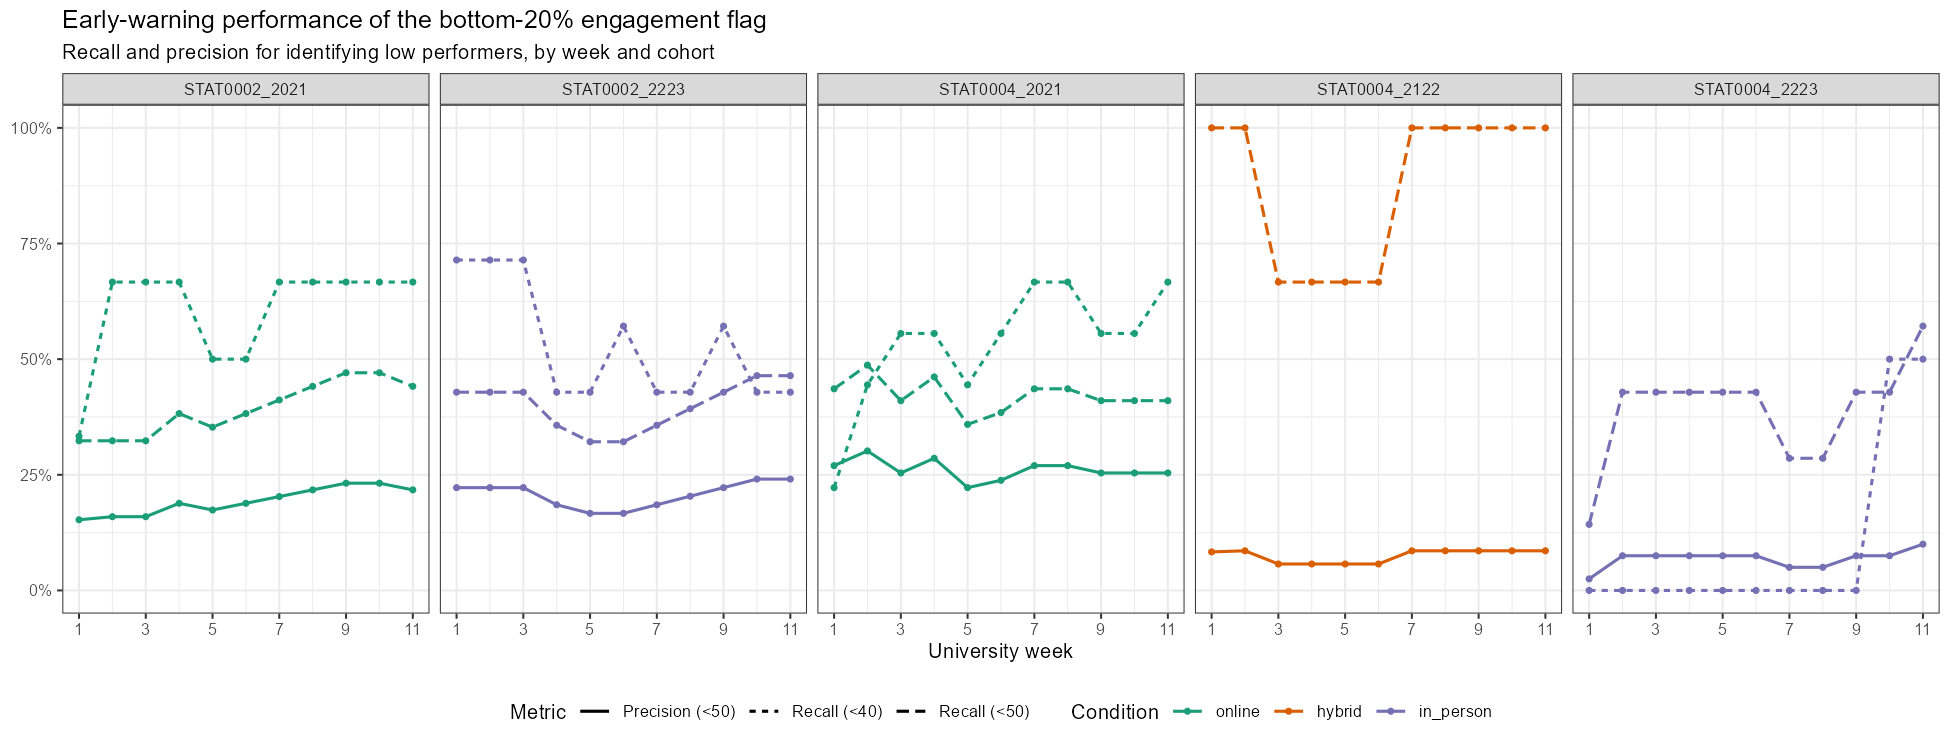
\includegraphics[width=0.95\textwidth]{08_recall_precision.png}
\caption{Recall and precision for the bottom engagement quintile across weeks.
Modest precision implies that most flagged students may still achieve passing
grades.}
\label{fig:earlywarn}
\end{figure}

\subsection{Boundary condition: delivery period and cohort confounding}
Because delivery condition is inseparable from cohort and year in this dataset,
comparisons across online, hybrid and in-person periods are best treated as a
descriptive boundary check rather than a test of delivery effects. Meta-analytic
moderator tests do not suggest that delivery label explains between-cohort
variation (all $p > 0.87$; Table~\ref{tab:meta}), and weekly correlations appear
broadly overlapping across periods (Figure~\ref{fig:crossmod}). This should not
be interpreted as evidence that delivery mode is irrelevant. Module design,
assessment structure, cohort composition and Moodle resource organisation may be
at least as important as the delivery label itself.

\begin{figure}[H]
\centering
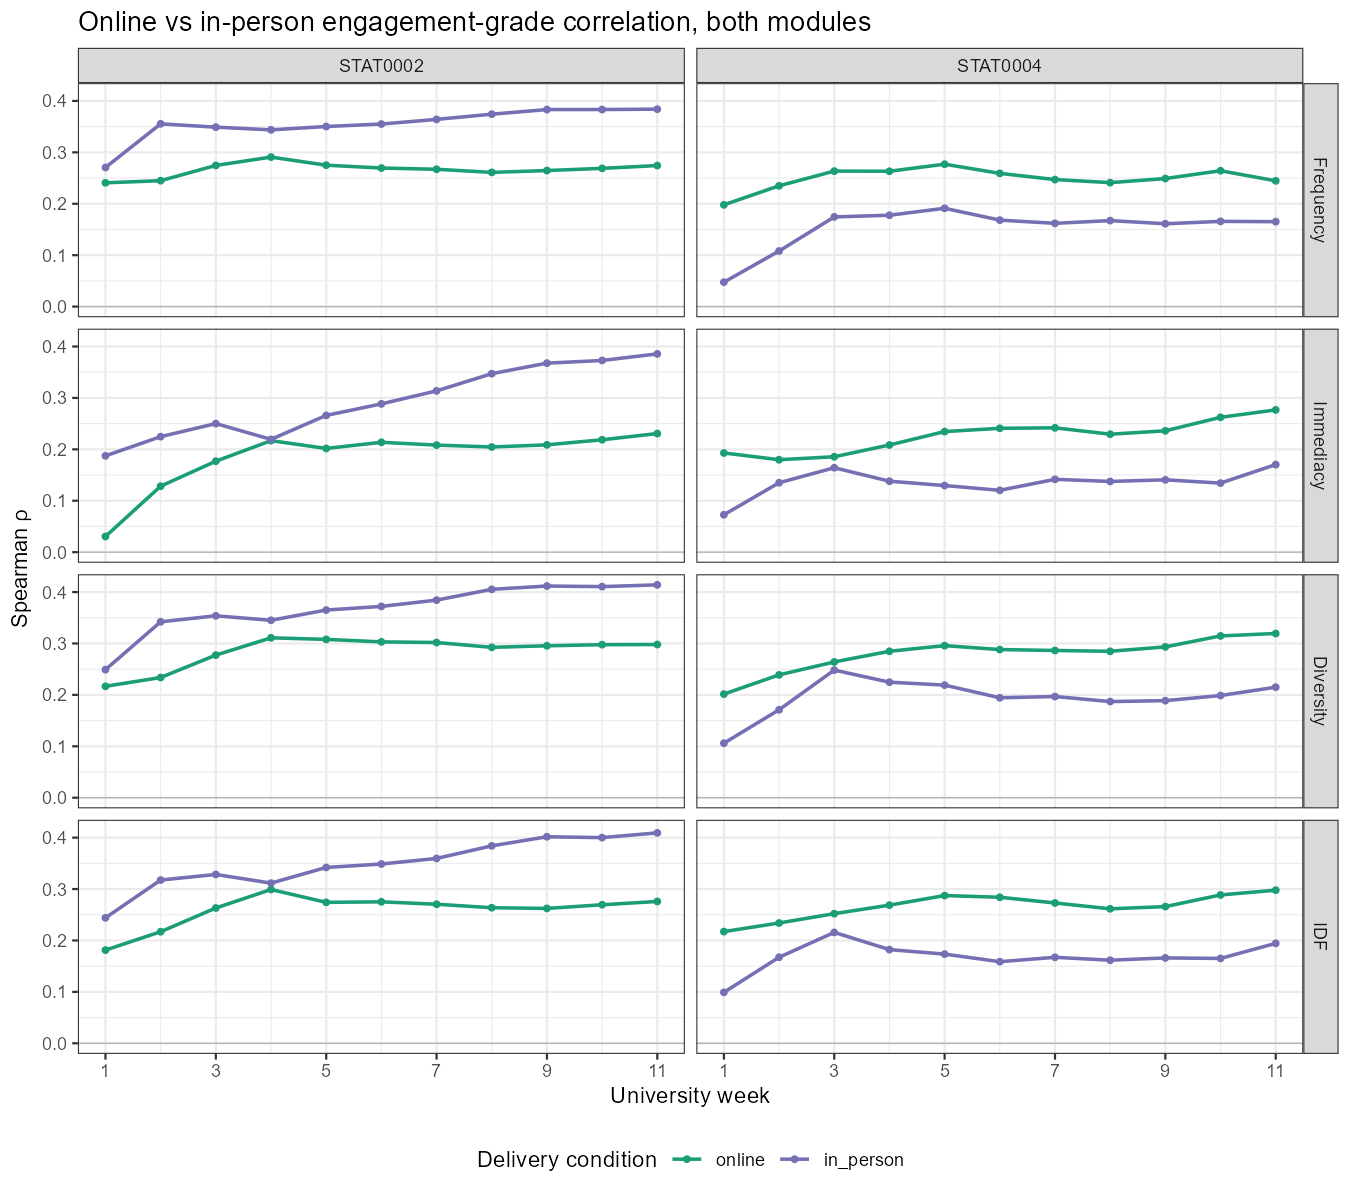
\includegraphics[width=0.95\textwidth]{09_cross_module_weekly.png}
\caption{Weekly engagement--grade correlation by module and delivery period.
Comparisons are descriptive; condition is confounded with academic year.}
\label{fig:crossmod}
\end{figure}

\subsection{Robustness checks}
Each check addressed a specific threat to the headline conclusions. Programme
adjustment tests whether the pooled engagement slope reflects degree-programme
composition rather than study behaviour itself; the slope changes by at most
14\%, so programme mix is not driving the result. False-discovery-rate correction
using the Benjamini--Hochberg procedure guards against spurious weekly
associations from repeated testing across weeks and indicators; 205 of 220 tests
remain significant. Alternative bounded-outcome specifications address skew and
ceiling effects in grade distributions and agree in sign with the main models in
all five cohorts. Finally, varying the at-risk engagement threshold examines
whether early-warning conclusions depend on an arbitrary quintile cut-off; recall
and precision shift in the expected direction without changing the overall
interpretation.

\section{Discussion}
\subsection{Interpretation of the component and distributional findings}
The central contribution of this report is not that Moodle activity predicts
grades perfectly: it does not. Rather, it shows that a transparent,
chapter-aligned summary of observed engagement retains a moderate relationship
with final performance in cohorts independent of the original validation. The
pooled association ($r=0.32$) and positive direction in every cohort extend the
evidence of \citet{johnston2025}, while also illustrating a central caution in
learning analytics: trace data are indicators of observable behaviour, not direct
measures of learning, motivation or effort \citep{winne2020,motz2019}.

Once the overlap among Frequency, Immediacy and Diversity is taken into account,
Diversity and Immediacy carry more unique information about final grades than
Frequency. This does not imply that session frequency is unimportant. Instead, it
suggests that repeated access alone is an incomplete account of productive online
study. Breadth of resource use is consistent with curriculum coverage, while
prompt first access is consistent with keeping pace with the intended teaching
sequence. This interpretation accords with work showing that frequency,
immediacy and regularity capture complementary aspects of online engagement
\citep{hoffman2023,you2016}. The contrast between similar bivariate correlations
and unequal relative-importance shares also demonstrates why component
interpretation should not rely only on individual correlations.

The quantile results add a distributional qualification. Engagement is associated
with grade throughout the cohort, but the association is larger among students in
the lower tail of the grade distribution. This is an empirical finding of the
present analysis rather than evidence that increasing Moodle engagement would
cause grades to rise by the estimated amount. It nevertheless supports treating
low observed engagement as one input to supportive outreach for students who may
be academically vulnerable, rather than as a tool for ranking all students with
the same confidence.

\subsection{Portability, trajectories and diagnostic value}
The metric performs differently across the two modules. The stronger
engagement--grade associations in STAT0002 than in STAT0004 are plausible given
differences in assessment structure, student autonomy and the extent to which
study activity occurs outside Moodle. Such contextual variation is expected:
the validity and utility of activity logs depend on instructional conditions and
course design \citep{gasevic2016,motz2019}. It reinforces the need to validate
the metric locally rather than assume that a threshold or effect size transfers
unchanged to every module.

The extension analyses clarify what is gained by retaining the temporal structure
of engagement. Low-steady, mid-variable and high-steady trajectories separate
final grades more sharply than a single score at one time point, in line with
evidence that longitudinal engagement profiles can reveal meaningful differences
in learning outcomes \citep{saqr2021,cerezo2016}. Regularity features add
information in STAT0002 but not in STAT0004, which is informative rather than a
failure: it indicates that temporal patterns should be treated as context-specific
diagnostic features. Similarly, stronger correlations with individually assessed
components than with peer- or group-marked outcomes are consistent with the fact
that group marks do not map cleanly onto individual study behaviour
\citep{almond2009}.

\subsection{Implications for early support}
The bottom-engagement flag identifies students with low \emph{observed} Moodle
engagement, not students who will fail. With precision of about 15--26\% at the
course midpoint in STAT0002, most flagged students may still pass. This trade-off
is common in early-warning systems and should determine the intensity of any
response \citep{conijn2017,akcapinar2019}. Appropriate uses are broad, low-cost
actions such as study reminders, non-accusatory check-ins, invitations to office
hours, human review, or dashboard-level monitoring of chapters and resources.
Engagement should be combined with coursework information, attendance where
available, tutor knowledge and student self-report before substantive action.

The component and trajectory results make this approach more informative than a
single risk label. A student may be behind the release schedule (low Immediacy),
using only a narrow range of materials (low Diversity), engaging irregularly, or
following a persistently low trajectory. From week~4 onward, the trajectory
analysis can identify a sustained low-engagement pattern with substantially higher
precision than the bottom-quintile rule identifies eventual low performance.
These distinctions can guide supportive, proportionate outreach. They do not
justify punitive messaging, high-stakes ranking, or an assumption that low Moodle
activity means low effort.

\subsection{Limitations}
The findings are associational and their scope is limited. Delivery condition is
perfectly confounded with academic year and cohort, so the data cannot identify
causal effects of online, hybrid or in-person delivery. The analysis covers two
statistics modules and five deliveries; external validity therefore remains to be
tested across disciplines, assessment designs and institutional contexts. Moodle
logs capture online behavioural engagement only, leaving offline study,
motivation, cognitive engagement and accessibility constraints unobserved
\citep{martinborup2022,nkomo2021}. Final grades are imperfect outcome measures,
especially when group, peer or non-invigilated assessment contributes. Small
numbers of low-performing students in some cohorts also make early-warning
estimates unstable. Finally, the metric depends on reliable chapter labelling and
resource organisation. Any operational deployment should therefore include local
validation of data quality, association strength and intervention thresholds.

\section{Conclusion}
This report validates an existing real-time Moodle engagement metric on new
STAT0002 and STAT0004 cohorts spanning online, hybrid and in-person delivery
periods. Cumulative engagement is moderately associated with final grades
($r=0.32$ pooled). Two findings receive particular emphasis. \textbf{First},
decomposing engagement into Frequency, Immediacy and Diversity shows that
breadth and promptness of resource use outweigh raw session frequency once
indicator overlap is removed, a distinction that bivariate correlations alone
would not reveal. \textbf{Second}, quantile regression shows that engagement
matters more for lower-performing students than for the average student,
supporting targeted support for at-risk learners rather than uniform prediction
across the grade distribution. Trajectory classes, temporal regularity and
assessment-component alignment provide additional diagnostic context. Delivery
comparisons are descriptive only. The metric should be used for low-cost
supportive monitoring with local validation, not high-stakes prediction.

\begin{thebibliography}{99}
\bibitem[Akçapınar et al.(2019)]{akcapinar2019}
Akçapınar, G., Altun, A., \& Aşkar, P. (2019). Using learning analytics to
develop early-warning system for at-risk students. \textit{International Journal
of Educational Technology in Higher Education}, 16, 40.

\bibitem[Almond(2009)]{almond2009}
Almond, R.~J. (2009). Group assessment: Comparing group and individual
undergraduate module marks. \textit{Assessment \& Evaluation in Higher
Education}, 34(2), 141--148.

\bibitem[Cerezo et al.(2016)]{cerezo2016}
Cerezo, R., Sánchez-Santillán, M., Paule-Ruiz, M.~P., \& Núñez, J.~C. (2016).
Students' LMS interaction patterns and their relationship with achievement: A
case study in higher education. \textit{Computers \& Education}, 96, 42--54.

\bibitem[Chong and Wong(2019)]{chong2019}
Chong, S., \& Wong, A. (2019). Proxy variables of online engagement on the learning
management system. \textit{International Journal of Learning and Teaching}, 296--300.

\bibitem[Conijn et al.(2017)]{conijn2017}
Conijn, R., Snijders, C., Kleingeld, A., \& Matzat, U. (2017). Predicting student
performance from LMS data: A comparison of 17 blended courses using Moodle LMS.
\textit{IEEE Transactions on Learning Technologies}, 10(1), 17--29.

\bibitem[Fincham et al.(2019)]{fincham2019}
Fincham, E., Whitelock-Wainwright, A., Kovanović, V., Joksimović, S., Van
Staalduinen, J.-P., \& Gašević, D. (2019). Counting clicks is not enough:
Validating a theorized model of engagement in learning analytics. In
\textit{Proceedings of the 9th International Conference on Learning Analytics
\& Knowledge} (pp.~501--510).

\bibitem[Fredricks et al.(2004)]{fredricks2004}
Fredricks, J.~A., Blumenfeld, P.~C., \& Paris, A.~H. (2004). School engagement:
Potential of the concept, state of the evidence. \textit{Review of Educational
Research}, 74(1), 59--109.

\bibitem[Gašević et al.(2016)]{gasevic2016}
Gašević, D., Dawson, S., Rogers, T., \& Gasevic, D. (2016). Learning analytics
should not promote one size fits all: The effects of instructional conditions in
predicting academic success. \textit{The Internet and Higher Education}, 28,
68--84.

\bibitem[Henrie et al.(2015)]{henrie2015}
Henrie, C.~R., Halverson, L.~R., \& Graham, C.~R. (2015). Measuring student
engagement in technology-mediated learning: A review. \textit{Computers \&
Education}, 90, 36--53.

\bibitem[Hoffman et al.(2023)]{hoffman2023}
Hoffman, D.~L., Furutomo, F., Eichelberger, A., \& McKimmy, P. (2023). Matters
of frequency, immediacy and regularity: Engagement in an online asynchronous
course. \textit{Innovative Higher Education}, 48, 655--677.

\bibitem[Koenker and Bassett(1978)]{koenker1978}
Koenker, R., \& Bassett, G. (1978). Regression quantiles.
\textit{Econometrica}, 46(1), 33--50.

\bibitem[Johnston et al.(2025)]{johnston2025}
Johnston, L.~J., Griffin, J.~E., Manolopoulou, I., \& Jendoubi, T. (2025). A
real-time metric of online engagement monitoring. \textit{arXiv preprint}
arXiv:2507.12162.

\bibitem[Lindeman et al.(1980)]{lindeman1980}
Lindeman, R.~H., Merenda, P.~F., \& Gold, R.~Z. (1980). \textit{Introduction to
bivariate and multivariate analysis}. Scott, Foresman.

\bibitem[Martin and Borup(2022)]{martinborup2022}
Martin, F., \& Borup, J. (2022). Online learner engagement: Conceptual
definitions, research themes, and supportive practices. \textit{Educational
Psychologist}, 57(3), 162--177.

\bibitem[Motz et al.(2019)]{motz2019}
Motz, B., Quick, J., Schroeder, N., Zook, J., \& Gunkel, M. (2019). The validity
and utility of activity logs as a measure of student engagement. In
\textit{Proceedings of the 9th International Conference on Learning Analytics
\& Knowledge} (pp.~300--309).

\bibitem[Nkomo et al.(2021)]{nkomo2021}
Nkomo, L.~M., Daniel, B.~K., \& Butson, R.~J. (2021). Synthesis of student
engagement with digital technologies: A systematic review of the literature.
\textit{International Journal of Educational Technology in Higher Education},
18, 34.

\bibitem[Proust-Lima et al.(2017)]{proustlima2017}
Proust-Lima, C., Philipps, V., \& Liquet, B. (2017). Estimation of extended mixed
models using latent classes and latent processes: The R package lcmm.
\textit{Journal of Statistical Software}, 78(2), 1--56.

\bibitem[Saqr and López-Pernas(2021)]{saqr2021}
Saqr, M., \& López-Pernas, S. (2021). The longitudinal trajectories of online
engagement over a full program. \textit{Computers \& Education}, 175, 104325.

\bibitem[Steiger(1980)]{steiger1980}
Steiger, J.~H. (1980). Tests for comparing elements of a correlation matrix.
\textit{Psychological Bulletin}, 87(2), 245--251.

\bibitem[Viechtbauer(2010)]{viechtbauer2010}
Viechtbauer, W. (2010). Conducting meta-analyses in R with the metafor package.
\textit{Journal of Statistical Software}, 36(3), 1--48.

\bibitem[Winne(2020)]{winne2020}
Winne, P.~H. (2020). Construct and consequential validity for learning analytics
based on trace data. \textit{Computers in Human Behavior}, 112, 106457.

\bibitem[You(2016)]{you2016}
You, J.~W. (2016). Identifying significant indicators using LMS data to predict
course achievement in online learning. \textit{The Internet and Higher
Education}, 29, 23--30.
\end{thebibliography}

\end{document}
